\documentclass{standalone}
\usepackage{graphicx}	
\usepackage{amssymb, amsmath, amsthm}
\usepackage{color}

\usepackage{tikz}
\usetikzlibrary{intersections, backgrounds, math}

\definecolor{light}{RGB}{220, 188, 188}
\definecolor{mid}{RGB}{185, 124, 124}
\definecolor{dark}{RGB}{143, 39, 39}
\definecolor{highlight}{RGB}{180, 31, 180}
\definecolor{darkteal}{RGB}{29, 79, 79}
\definecolor{darkolive}{RGB}{97, 123, 45}
\definecolor{gray10}{gray}{0.1}
\definecolor{gray20}{gray}{0.2}
\definecolor{gray30}{gray}{0.3}
\definecolor{gray40}{gray}{0.4}
\definecolor{gray60}{gray}{0.6}
\definecolor{gray70}{gray}{0.7}
\definecolor{gray80}{gray}{0.8}
\definecolor{gray90}{gray}{0.9}
\definecolor{gray95}{gray}{0.95}

\tikzmath{
  function normal(\x) {
    return exp(-0.5 * \x * \x);
  };
  function laplace(\x) {
    return exp(-sqrt(\x * \x));
  };
  function cauchy(\x) {
    return 1 / (1 + \x * \x));
  };
}

\begin{document}

\begin{tikzpicture}[scale=0.45, thick]
  
\begin{scope}[shift={(0, 0)}]
  \draw[white] (-9, -7) rectangle (9, 6);
    
  \begin{scope}
    \clip (-7, -7) rectangle (7, 6);
        \node at (0, 0) {\includegraphics[width=4.5cm]{heavy_density_comp.eps}};
  \end{scope}
  
  
  \draw [<->, >=stealth, line width=1] (-5 - 0.025, -5) -- +(10, 0);
  \node[] at (0, -6) { $\theta_{k}$ };
  
  \node[light, align=center] at (-5.5, -1.65) { $1$ };
  
  \node[light, align=center] at (-0.6, 5) { $-\tau$ };
  \node[light, align=center] at (0.15, 5.5) { $0$ };
  \node[light, align=center] at (0.7, 5) { $\tau$ };
  
  \draw [->, >=stealth, line width=1] (-5, -5 - 0.025) -- +(0, 10);
  \node[rotate=90,align=center] at (-7.5, 0) { Horseshoe Density Function/\\Cauchy Density Function };
  
\end{scope}
  
\end{tikzpicture}

\end{document}  